


\tikzset{every picture/.style={line width=0.75pt}} %set default line width to 0.75pt        

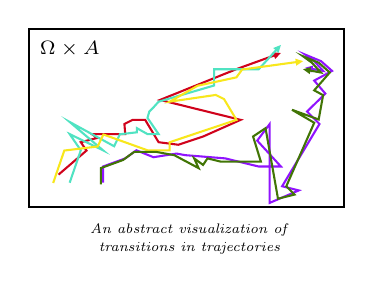
\begin{tikzpicture}[x=0.75pt,y=0.75pt,yscale=-1,xscale=1]
%uncomment if require: \path (0,1974); %set diagram left start at 0, and has height of 1974

%Shape: Rectangle [id:dp10581972605309897] 
\draw  [fill={rgb, 255:red, 255; green, 255; blue, 255 }  ,fill opacity=1 ] (189.9,1694) -- (342,1694) -- (342,1779.89) -- (189.9,1779.89) -- cycle ;
%Straight Lines [id:da15954508078344698] 
\draw [color={rgb, 255:red, 208; green, 2; blue, 27 }  ,draw opacity=1 ]   (308.57,1706.73) -- (290.18,1713.38) -- (253.16,1728.29) -- (292,1737.89) -- (274,1745.89) -- (262,1749.89) -- (252.48,1748.66) -- (246,1737.89) -- (240,1737.89) -- (236,1739.89) -- (236.41,1744.75) -- (220.34,1744.75) -- (222.9,1746.61) -- (214.99,1748.66) -- (217.75,1752.68) -- (204.28,1764.27) ;
\draw [shift={(311.39,1705.71)}, rotate = 160.12] [fill={rgb, 255:red, 208; green, 2; blue, 27 }  ,fill opacity=1 ][line width=0.08]  [draw opacity=0] (3.57,-1.72) -- (0,0) -- (3.57,1.72) -- cycle    ;
%Straight Lines [id:da4456358262502481] 
\draw [color={rgb, 255:red, 80; green, 227; blue, 194 }  ,draw opacity=1 ]   (309.37,1704.02) -- (300.68,1713.52) -- (279.26,1713.52) -- (279.26,1721.33) -- (252.48,1729.14) -- (250,1731.89) -- (248,1733.89) -- (247.12,1736.94) -- (252.48,1744.75) -- (247.12,1744.75) -- (242,1741.89) -- (242,1743.89) -- (233.84,1744.83) -- (231.05,1750.61) -- (209.63,1738.9) -- (225.7,1752.56) -- (209.63,1744.75) -- (214.99,1752.56) -- (209.63,1768.18) ;
\draw [shift={(311.39,1701.81)}, rotate = 132.45] [fill={rgb, 255:red, 80; green, 227; blue, 194 }  ,fill opacity=1 ][line width=0.08]  [draw opacity=0] (3.57,-1.72) -- (0,0) -- (3.57,1.72) -- cycle    ;
%Straight Lines [id:da9735384751024792] 
\draw [color={rgb, 255:red, 248; green, 231; blue, 28 }  ,draw opacity=1 ]   (319.13,1710.02) -- (292.73,1713.64) -- (289.97,1717.42) -- (271.3,1721.45) -- (257.83,1729.14) -- (280,1725.89) -- (284,1727.89) -- (290,1737.89) -- (257.83,1748.66) -- (257.83,1752.56) -- (247.12,1752.56) -- (225.89,1744.95) -- (223.1,1750.73) -- (207.04,1752.68) -- (201.68,1768.3) ;
\draw [shift={(322.1,1709.62)}, rotate = 172.2] [fill={rgb, 255:red, 248; green, 231; blue, 28 }  ,fill opacity=1 ][line width=0.08]  [draw opacity=0] (3.57,-1.72) -- (0,0) -- (3.57,1.72) -- cycle    ;
%Straight Lines [id:da9773846199264294] 
\draw [color={rgb, 255:red, 144; green, 19; blue, 254 }  ,draw opacity=1 ]   (326.12,1713.28) -- (331.74,1714.3) -- (327.46,1709.62) -- (323.17,1706.49) -- (330.76,1709.62) -- (336.03,1714.3) -- (327.46,1718.99) -- (332.81,1725.23) -- (324,1733.89) -- (330,1739.89) -- (312,1769.89) -- (320,1771.89) -- (306,1777.89) -- (306,1739.89) -- (300,1747.89) -- (311.39,1760.37) -- (300.68,1760.37) -- (294.88,1758.96) -- (291.82,1758.21) -- (287.47,1757.16) -- (284.61,1756.46) -- (273.86,1755.59) -- (265.33,1754.9) -- (261.13,1754.14) -- (250,1755.89) -- (241.77,1752.56) -- (236.41,1756.46) -- (225.7,1760.37) -- (225.7,1768.18) ;
\draw [shift={(323.17,1712.74)}, rotate = 10.33] [fill={rgb, 255:red, 144; green, 19; blue, 254 }  ,fill opacity=1 ][line width=0.08]  [draw opacity=0] (3.57,-1.72) -- (0,0) -- (3.57,1.72) -- cycle    ;
%Straight Lines [id:da5869208077424531] 
\draw [color={rgb, 255:red, 65; green, 117; blue, 5 }  ,draw opacity=1 ]   (325.05,1714.06) -- (330.67,1715.08) -- (326.39,1710.4) -- (322.1,1707.27) -- (329.69,1710.4) -- (334.95,1715.08) -- (327.46,1723.67) -- (331.74,1726.01) -- (329.6,1737.72) -- (316.75,1733.04) -- (327.46,1739.29) -- (314,1769.89) -- (318,1773.89) -- (310,1775.89) -- (304,1741.89) -- (298,1745.89) -- (301.75,1758.03) -- (288.9,1758.03) -- (282.47,1758.03) -- (276.04,1756.46) -- (273.9,1759.59) -- (269.62,1756.46) -- (271.76,1761.15) -- (260.06,1754.92) -- (251.41,1753.34) -- (240.69,1753.34) -- (235.34,1757.24) -- (224.63,1761.15) -- (224.63,1768.96) ;
\draw [shift={(322.1,1713.52)}, rotate = 10.33] [fill={rgb, 255:red, 65; green, 117; blue, 5 }  ,fill opacity=1 ][line width=0.08]  [draw opacity=0] (3.57,-1.72) -- (0,0) -- (3.57,1.72) -- cycle    ;


% Text Node
\draw (209.73,1703.84) node  [font=\scriptsize] [align=left] {$\displaystyle \Omega \times A$};
% Text Node
\draw (267.61,1790.89) node   [align=left] {{\tiny \textit{An abstract visualization of}}};
\draw (267.61,1800) node   [align=left] {{\tiny \textit{transitions in trajectories}}};

\end{tikzpicture}